\paragraph{high\_degree\_interpolation}

InterpolationGate is used for interpolation a polynomial, whose points are a (base field) coset of the multiplicative subgroup 
with the given size, and whose values are extension field elements. As for HighDegreeInterpolationGate,  allows constraints of variable degree, 
up to \verb|1 << subgroup_bits|. The higher degree is a tradeoff for less gates (than LowDegreeInterpolationGate).


HighDegreeInterpolationGate trace is shown in \figref{fig:high-degree-interpolation}.

\begin{figure}[!ht]
    \centering
    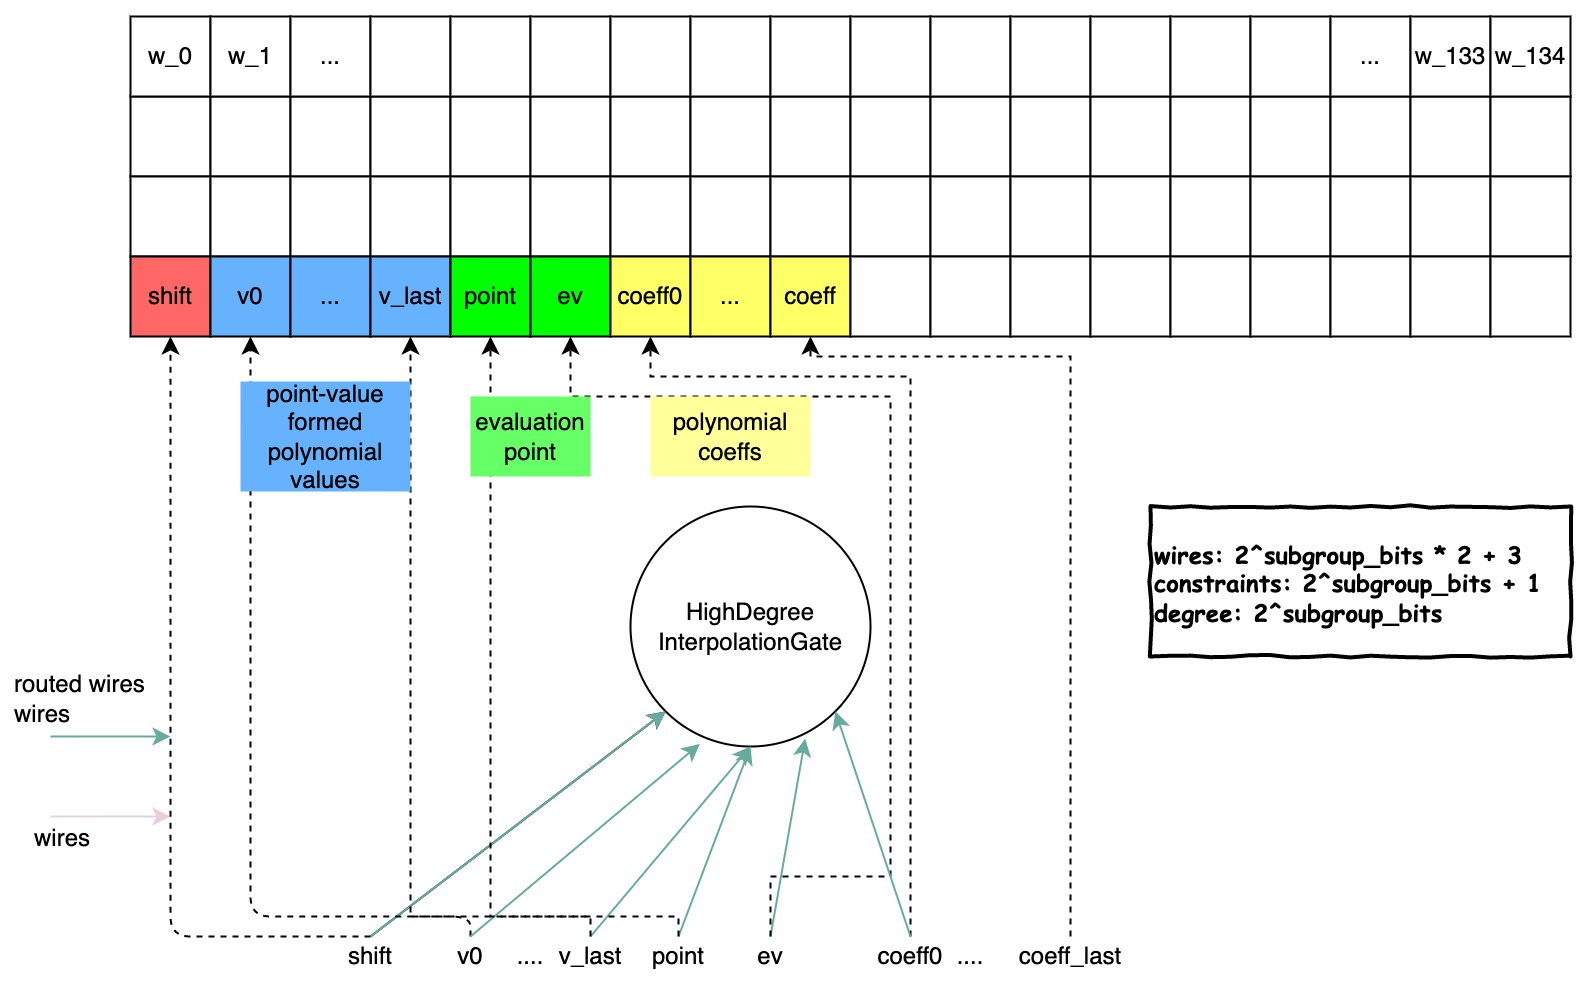
\includegraphics[width=0.8\textwidth]{gates/high_degree_interpolation.jpeg}
    \caption{HighDegreeInterpolationGate}
    \label{fig:high-degree-interpolation}
\end{figure}


Constraints:
\begin{itemize}
    \item Bring each point(from the point-value pairs) into the coefficient polynomial to compute the computed\_value, 
    and compare the constraint with the value(from the point-value pairs). -- A total of $2^{\text{subgroup\_bits}}$ constraints.
    \begin{lstlisting}
for (i, point) in coset.into_iter().enumerate() {
    let value = vars.get_local_ext_algebra(self.wires_value(i));
    let computed_value = interpolant.eval_base(point);
    constraints.extend((value - computed_value).to_basefield_array());
}
    \end{lstlisting}
    coset: $[sg, sg^2,...,sg^{2^{\text{subgroup\_bits}}}], \ s=\text{shift}$
    \item Evaluate the coefficient-form polynomial at evaluation point, and constrain with ev. -- 1 constraint.
\end{itemize}

The degree of this gate equals the number of points (num\_points): max point power is $\text{num\_points} - 1$, and multiplication by coefficient adds 1 degree.

Number of constraints equals $\text{num\_points} + 1$: num\_points for consistency between the coefficients and the point-value pairs, 1 constraints for the evaluation value. 
